\documentclass[a4paper, 12pt, twoside, final, book, russian, fittopage, cyremdash, openright]{ncc}
\usepackage[a4paper]{geometry}
\geometry{verbose, tmargin=3cm, bmargin=3cm, lmargin=2cm, rmargin=1.5cm, headheight=1cm, headsep=1cm, footskip=1.5cm}
\usepackage[T2A]{fontenc}
\usepackage[utf8]{inputenc}
\usepackage{wrapfig}
\usepackage[section]{placeins}
\usepackage{booktabs}
\usepackage{longtable}
\usepackage{hyperref}
\usepackage{xspace}
\usepackage[headings]{ncchdr}
\usepackage{ncccomma}
\usepackage{desclist}
\usepackage{indentfirst}
\usepackage{upgreek}
\usepackage{marvosym}
\usepackage{multirow}
\usepackage{amsfonts}
\usepackage{enumerate}
\usepackage{rotating}
\usepackage{array}
\usepackage{graphicx}
\usepackage[font=small]{caption}
\usepackage{xfrac}
\usepackage{accents}
\usepackage[inline]{enumitem}

\makeindex

\clubpenalty=10000
\widowpenalty=10000

\righthyphenmin=2 % разрешаем переносить два последних символа

\renewcommand{\bfdefault}{b} % плотный жирный

\newcommand{\mps}{~м/с\xspace}
\newcommand{\kph}{~км/ч\xspace}
\newcommand{\otdo}{\,\ensuremath{\div}\,}
\newcommand{\gr}{\ensuremath{\,^\circ}\xspace}
\newcommand{\grC}{\ensuremath{\,^\circ{}C}\xspace}

\graphicspath{{pics/}}

\begin{document}

\author{\LARGE С.\=,Ю.~Зиновьев}
\title{Составление прогноза погоды по местным признакам}
\setyear{....}
\titlefoot{\theyear}
\maketitle


\frontmatter

{\small \tableofcontents}
{\small \listoffigures}
{\small \listoftables}

\openrightorany

\chapter*{Введение}

Погода для мореплавателей \--- прежде всего фактор, определяющий
безопасность плавания. Затем \--- фактор экономический, и, наконец,
как и для всех людей, \--- фактор комфорта, самочувствия и
здоровья. Предсказание погоды, с научной точки зрения, одна из
сложнейших физических задач. Для её решения существует несколько
методов.

Гидрометеорологическая обстановка \--- это метеорологические и
гидрологические условия\footnote{Содержание, порядок составления и
  оценки прогноза гидрологической обстановки определяются специальными
  документами}, складывающиеся в районах океанов и морей под
воздействием процессов, происходящих в атмосфере и океане и
оказывающих влияние на действия сил, применение оружия и технических
средств Военно-Морского Флота.

Анализ фактической и предсказание (расчёт) ожидаемой метеорологической
обстановки необходимы для учёта влияния этой обстановки при
планировании операций (действий) и управлении силами флота.

Анализ фактической и предсказание (расчёт) ожидаемой метеорологической
обстановки необходимы для учёта влияния этой обстановки при
планировании операций (действий) и управлении силами флота.

Под прогнозом метеорологической обстановки (прогнозом погоды)
понимается научно обоснованное предсказание значений метеорологических
элементов и явлений на определённый район и заданный промежуток
времени. Прогноз является конечным результатом анализа атмосферных
процессов, который проводится на основе данных о фактической
метеорологической обстановке и известных физических закономерностей в
развитии атмосферных процессов.

\mainmatter

\chapter{Основные понятия гидрометеорологического обеспечения безопасности плавания}

Воздушный океан находится в постоянном движении.

\textbf{Воздушная масса}\index{воздушная масса} \--- достаточно
большое количество воздуха (высотой от 1~до 10~километров и
горизонтальной протяжённостью до нескольких тысяч километров)
сравнительно однородного по своим физическим свойствам и резко
отличного от воздуха соседних районов. В зависимости от
географического расположения очагов их формирования и подстилающей
поверхности воздушные массы получали названия: арктический морской
(континентальный) воздух, воздух умеренных широт морской
(континентальный), тропический морской (континентальный) воздух,
экваториальный воздух.

Вес столба воздуха, распределённого на единице площади, называют
давлением\index{давление}: плотный холодный воздух в приземном слое
создаёт высокое давление, а более тёплый и менее плотный воздух \---
низкое давление.

Разница в давлении между воздушными массами заставляет их двигаться из
области высокого давления к области низкого, но сила трения
подстилающей поверхности, вращение Земли и центробежная сила изменяют
траекторию движения воздушных масс.

\section{Ветер}
\label{sec:wind}

\textbf{Ветры}\index{ветер} \--- это движение потоков воздуха под
действием разности температур и
давлений. \textbf{Штормом}\index{шторм} называется продолжительный
сильный ветер, скорость которого превышает 15\mps{}.
\textbf{Шквалом}\index{шквал} называют внезапное усиление ветра до
штормового с резким изменением направления.
\textbf{Ураганом}\index{ураган} называется буря, когда скорость ветра
превышает 24\mps{}.

\section{Местные ветры}
\label{sec:local_winds}\index{местные ветры}

Под \textbf{местными ветрами} понимают воздушные течения небольшой
горизонтальной протяжённости (от нескольких сот метров до десятков
километров), характерные только для определённых географических
районов. Происхождение их различно. Местные ветры могут быть либо
проявлением местных циркуляции (бризы\index{бриз}, горно-долинные
ветры\index{горно-долинный ветер}), либо они представляют собой
изменения крупномасштабных движений атмосферы под влиянием орографии
местности (фен\index{фен}, бора\index{бора}). Кроме того, в некоторых
районах местными ветрами иногда называют сильные или обладающие
особыми свойствами ветры, которые по существу являются
крупномасштабными течениями. Подробно местные ветры описываются в
лоциях морей.

\section{Катабатические ветры}
\label{sec:catabatic_wind}

Вдоль холодного побережья Гренландии, Антарктиды и в некоторых других
местах наблюдаются так называемые \textbf{катабатические
  ветры}\index{катабатические ветры}, иногда достигающие штормовой
силы. Вследствие охлаждения воздуха он становится более плотным и под
действием силы тяжести стекает по склонам вниз к морю. К семейству
катабатических ветров относится также бора\index{бора}.

\section{Бора}
\label{sec:bora_wind}\index{бора}

\textbf{Бора} \--- это сильный и порывистый ветер, направленный вниз
по горному склону и приносящий в зимнее время значительное
похолодание. Бора наблюдается в местностях, где невысокий горный
хребет граничит с морем. Холодная воздушная масса, встречая на пути
горный хребет, задерживается им; происходит накопление воздуха перед
хребтом. Воздушная масса увеличивает свою вертикальную протяжённость
до момента, когда она сравняется с высотой перевала. После этого
холодный воздух через перевал обрушивается в сторону моря в виде
холодного, штормовой силы ветра. Вертикальная мощность боры обычно не
превышает 200\otdo{}500~м, а распространяется она в море на несколько
километров.

В Советском Союзе бора встречается во многих местах, но особой силы
она достигает в зимнее время в районах Новороссийска и Новой Земли,
где скорость ветра в порывах достигает иногда 50\otdo{}60\mps. Бора
наблюдается также в районе Триеста.

Бора возникает как результат переваливания холодных масс воздуха через
горные хребты и их обвал к морю. Бора является типичным ветром для
западных берегов о.~Новой Земли, где её повторяемость зимой достигает
10\otdo{}11\%. Типичное синоптическое положение, обусловливающее бору,
сводится к наличию над юго-восточной частью Баренцева моря циклона,
перемещающегося на восток, при наличии над Карским морем и севером
Баренцева моря области повышенного давления.

Скорости ветра при боре нередко превышают 40\mps{}, а в порывах могут
достигать 60\mps{}.  Направление ветра при этом обычно восточное. Бора
может наблюдаться в течение нескольких суток и распространяется в море
на расстоянии до 20~миль.

Явления, подобные новоземельской боре, отмечаются также и в других
районах Северного театра. Они наблюдаются у юго-восточных, южных и
юго-западных берегов Гренландии достигая наибольшей повторяемости в
весеннее время года. В прибрежной полосе при боре скорости ветра могут
достигать 60\otdo{}80\mps{}. И распространяться в море на
30\otdo{}40~миль. Направление такого воздушного потока перпендикулярно
береговой черте и направлено в сторону моря.

\section{Смерчи}
\label{sec:tornados}

В условиях большой неустойчивости атмосферной стратификации, когда
образуются мощные кучево-дождевые облака, под ними возникают
вертикальные вихри небольшого диаметра, простирающиеся от поверхности
Земли до нижней границы облаков. Над морем такие вихри называют
\textbf{смерчами}\index{смерч}, а над сушей \---
\textbf{тромбами}\index{тромб}. В Северной Америке тромбы называются
\textbf{торнадо}\index{торнадо}.

Вихрь возникает в передней части грозового облака. У смерчей над морем
диаметр вихря достигает десятков метров, у тромбов над сушей \---
100\otdo{}200~м, а в американских торнадо \--- ещё больше. Скорость
вращения воздуха в таком вихре более 100\mps{}. Вращение воздуха
сопровождается поднятием его вверх по спирали. В процессе вращения
вихрь втягивает сверху облако, а снизу \--- воду или пыль с земной
поверхности. Поэтому смерчи и тромбы видны как тёмные столбы между
облаками и Землёй, расширяющиеся сверху и снизу.

Тромбы и смерчи перемещаются вместе с облаком со скоростью
30\otdo{}40\kph{}. Время существования смерчей \--- минуты, тромбов \---
десятки минут, но иногда несколько часов. За это время смерч может над
морем продвинуться на несколько миль, а тромб над сушей \--- на десятки
километров, сметая все на своём пути.

Тромб сопровождается грозой, ливневым дождём, градом. Водяные смерчи
реже связаны с грозами. Тромбы проходят поодиночке, хотя торнадо
изредка наблюдаются по два и более. Смерчи часто возникают целыми
сериями, по несколько вихрей, даже по 20\otdo{}30. Необходимым условием
возникновения вихрей являются высокая температура воздуха и его
большое влагосодержание. Эти условия характерны для атлантического
побережья Северной Америки.

Атмосферное давление в вихре сильно понижено, на десятки
миллибар. Падение давления при прохождении тромба настолько велико и
быстро, что внутреннее давление в зданиях не успевает выровняться с
наружным, поэтому дома, попавшие в сферу действия тромба, иногда
взрываются. Смерчи обладают меньшей разрушительной силой, однако суда
должны избегать встречи со смерчами, что сделать нетрудно, так как они
видны с достаточно большого расстояния.

\section{Тропические ураганы}
\label{sec:hurricans}\index{ураганы!тропические}

В северную часть Атлантического океана в отдельных случаях проникают
\textbf{тропические циклоны}\index{циклоны!тропические}, известные под
названием \textbf{вест-индских ураганов}\index{ураганы!вест-индские},
обладающих огромной разрушительной силой. Подсчитано, что если бы всю
энергию только одного тропического циклона превратить в электрическую,
то её хватило бы всему человечеству на несколько лет. В среднем за год
в Атлантическом океане наблюдается около 12\otdo{}13 циклонов. Они
характеризуются небольшими размерами, не превышающими в диаметре
100\otdo{}300~миль, низким давлением в центре, достигающим 940~мб,
большими барическими градиентами и скоростями ветра до
40\mps{}. Особенно сильный ветер наблюдается в центральной части
урагана, причём усиливается он внезапно. Таким образом, вест-индские
ураганы представляют собой чрезвычайно опасное явление для
мореплавателей и при их приближении должны быть приняты меры для
расхождения с центром урагана.  Иногда вест-индские ураганы имеют в
диаметре 1000 и более миль. В таких случаях ветер достигает большой
силы только в центральной части урагана диаметром несколько сот
миль. Сильный ветер, связанный с тропическим циклоном, развивает
большую волну, которая распространяется радиально по всем направлениям
и ощущается в виде зыби на больших расстояниях. \textit{Скорость
  распространения зыби больше скорости перемещения циклона, и поэтому
  её появление в направлении, не совпадающим с направлением дующего
  ветра, может служить одним из важнейших признаков приближения
  урагана}.

\section{Бризы}
\label{sec:breeze}

\textbf{Бризами}\index{бриз} называются реверсивные ветры на берегах
океанов, морей и озёр, имеющие суточную периодичность. У поверхности
Земли днем они направлены с моря на сушу \--- морские бризы, а ночью
\--- с суши на море \--- береговые бризы. В низких широтах бризы
образуются в течение всего года, в умеренных и высоких широтах —
обычно в тёплое время года.

\begin{figure*}[htb]
   \centering
   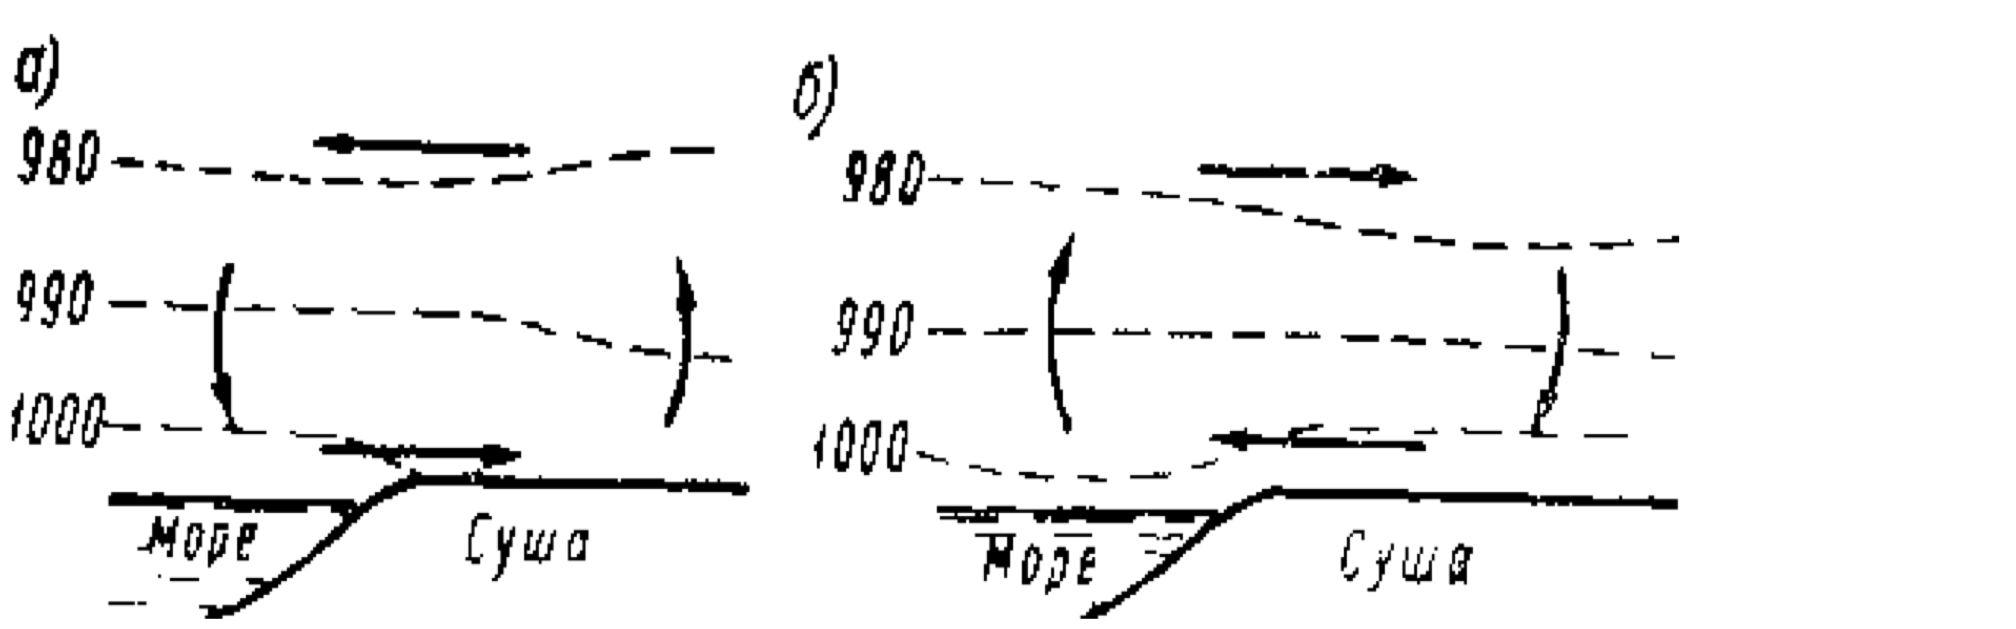
\includegraphics[scale=0.2]{01_breeze.png}
   \caption{Бризы}
   \label{fig:01_breeze}
   \centering{}
   \small
   a)~морской; б)~береговой
\end{figure*}

Причина возникновения бризов \--- неравномерное нагревание и
охлаждение суши и водной поверхности в течение суток. После восхода
Солнца поверхность суши и воздух над ней прогреваются значительно
быстрее, чем море. Так как в теплом воздухе давление с высотой падает
медленнее, чем в холодном, то по мере нагревания воздуха над сушей на
некоторой высоте давление будет выше, чем на той же высоте над
морем. Изобарические поверхности на высотах будут наклонены в сторону
моря, и вследствие этого на высотах начнётся отток воздуха с суши на
море (рис.~\ref{fig:01_breeze}). Благодаря увеличению массы воздуха
над морем давление в нижних слоях здесь окажется выше, чем над сушей,
т.е. изобарические поверхности здесь будут наклонены с моря на
сушу. Это приведёт к движению воздуха с моря на сушу, т.е. к развитию
ветра, называемого \textbf{морским
  бризом}\index{бриз!морской}. Морской бриз начинается с 8\otdo{}10~ч
утра. Постепенно он усиливается и достигает максимума после полудня,
затем медленно затухает ко времени захода Солнца.

Ночью поверхность суши охлаждается быстрее, чем поверхность моря,
вследствие чего на высотах движение воздуха будет происходить с моря к
суше, а в нижних слоях будет развиваться ветер от суши к морю,
называемый \textbf{береговым бризом}\index{бриз!береговой}. Береговой
бриз начинается после захода Солнца и продолжается до 8\otdo{}9~ч
следующего дня.

Морской бриз обычно сильнее берегового, так как в дневные часы
контраст температур между водной поверхностью и сушей значительно
больше, чем ночью.

Скорость ветра и вертикальные и горизонтальные размеры бризовой
циркуляции весьма разнообразны и изменчивы. Они зависят от суточного
хода температуры воздуха над континентом, а, следовательно, от широты
места, от градиентов давления, а также от рельефа и формы побережья.

Особенно чётко бризовая циркуляция проявляется в тропической зоне, где
контрасты температур между поверхностью суши и моря особенно велики.

Так, в тропической зоне морской бриз зарождается на расстоянии
100\otdo{}150~км от берега и проникает на сушу на 80\otdo{}100~км; береговой
бриз распространяется на меньшее расстояние. В умеренных широтах
морской бриз зарождается в 10\otdo{}100~км от берега, и в глубь суши он
распространяется до 30\otdo{}40~км. Скорость ветра при морских бризах в
тропической зоне достигает 5\otdo{}7\mps{}, при береговых \--- 1\otdo{}3\mps{}.

\section{Береговой эффект}
\label{sec:coast_effect}

Рассмотрим случай, когда ветер над морем дует параллельно береговой
черте, идущей, например, в меридиональном направлении. Так как ветер
над сушей отклоняется от изобар на больший угол, чем над морем, то
вдоль западного берега образуется \textbf{зона
  дивергенции}\index{дивергенции зона} (расходимость линий тока), в
которой происходит ослабление ветра, опускание масс воздуха, а
следовательно, устанавливается безоблачная погода. Наоборот, вдоль
восточного берега образуется \textbf{зона
  конвергенции}\index{конвергенции зона} (сходимость линий тока) и
соответственно будет происходить усиление ветра, развитие восходящих
движений воздуха, что способствует образованию облачности и выпадению
осадков. Такое изменение силы ветра называется \textbf{береговым
  эффектом}\index{береговой эффект}
(рис.~\ref{fig:02_coast_effect}. Ветер в прибрежной зоне всегда
усиливается, если суша располагается справа от направления линии тока
ветра, и ослабевает, если суша слева. Береговой эффект будет
наблюдаться и в случае, когда ветер дует под острым углом к береговой
черте. Этот эффект усиливается, если берег высокий или гористый.

\begin{figure*}[htb]
   \centering
   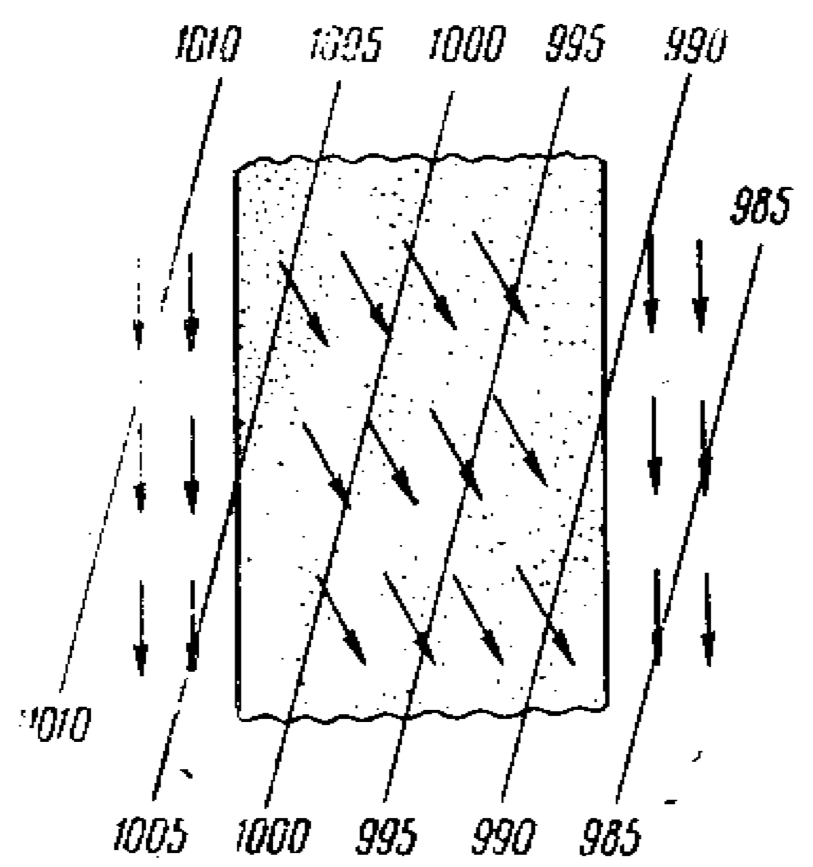
\includegraphics[scale=0.2]{02_coast_effect.png}
   \caption{Береговой эффект}
   \label{fig:02_coast_effect}
\end{figure*}

Всякое препятствие, стоящее на пути воздушного потока, отклоняет его,
и он либо обтекает препятствие с боков, либо перетекает через него
сверху. При горизонтальном обтекании ветер усиливается у мысов,
оконечностей островов и т.п., так как линии тока в таких местах
сближаются. Это усиление ветра называется \textbf{угловым
  эффектом}\index{угловой эффект}. Если мыс или остров остаётся справа
от направления линии тока, то ветер будет особенно сильным. Примером
является \textbf{бакинский норд}\index{бакинский норд} \--- ветер
северных направлений у Апшеронского полуострова на Каспийском море.

Существенное усиление ветра наблюдается в проливах с высокими
берегами, причём в них преобладают ветры, дующие вдоль пролива.  За
препятствиями скорость ветра уменьшается, и там образуется ветровая
тень. Этим объясняется известный факт, что в заливах, бухтах и фьордах
ветер значительно слабее, чем в открытом море.

\section{Изобары}
\label{sec:isobars}

\textbf{Изобарами}\index{изобары} называются линии, соединяющие на карте точки с равным атмосферным давлением.

\section{Барическое поле}
\label{sec:baric_field}

\textbf{Барическое поле}\index{барическое поле} \--- распределение давлений на каком-либо горизонтальном уровне.

\section{Формы барического рельефа}
\label{sec:baric_relief}

\textbf{Формы барического рельефа}\index{барического рельефа форма}
\--- системы расположения изобар, характеризующие тип падения или
повышения давления. Различают следующие формы барического рельефа:
\textbf{циклон}, \textbf{ложбина}, \textbf{антициклон},
\textbf{отрог}, \textbf{гребень} или \textbf{клин},
\textbf{седловина}.

\section{Барическая тенденция}
\label{sec:baric_tendency}

\textbf{Барическая тенденция}\index{барическая тенденция} \--- это
величина изменения давления в течении трёх часов перед последним
наблюдением.

\section{Барический закон ветра}
\label{sec:baric_wind_law}

\textbf{Барический закон ветра}\index{барический закон ветра} \---
если встать спиной к ветру, то в северном полушарии низкое давление
находится слева, а высокое \--- справа от направления ветра. В южном
полушарии \--- наоборот.

\section{Циклон}
\label{sec:cyclon}

\begin{figure*}[htb]
   \centering
   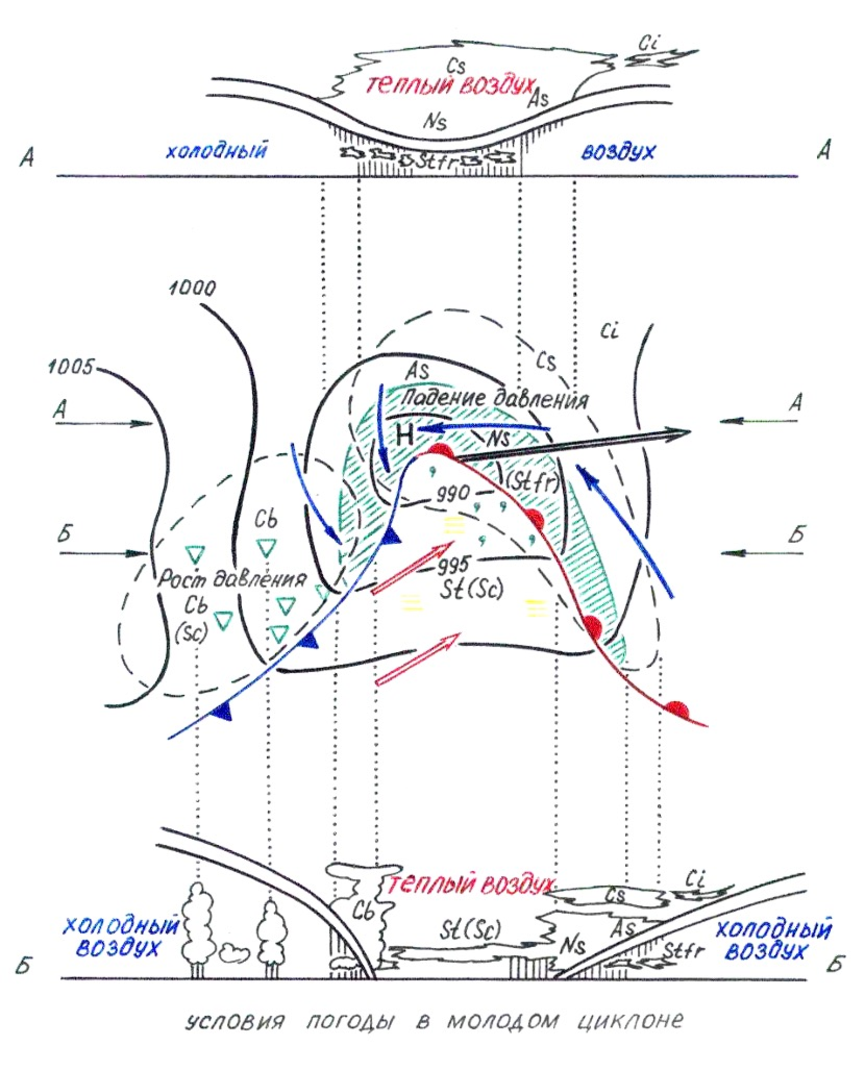
\includegraphics[scale=1.0]{03_cyclon.pdf}
   \caption{Условия погоды в молодом циклоне}
   \label{fig:03_cyclon}
\end{figure*}


\textbf{Циклон}\index{циклон} \--- вихреобразное возмущение в
атмосфере с понижающимся давлением к центру. Характеризуется системой
ветров, дующих против часовой стрелки в северном полушарии и по
часовой стрелке в южном полушарии. Циклон зарождается, когда область
пониженного давления возникает на границе двух масс воздуха разной
температуры. В циклонах два фронта \--- холодный и тёплый. Стадии
развития циклона: волна, волновой циклон, окклюзия или замыкание,
вихрь.

Стадия молодого циклона (рис.~\ref{fig:03_cyclon}) характеризуется
наличием тёплого сектора, т.е. сектора в южной части депрессии с
тёплым воздухом и ограниченного спереди тёплым фронтом, сзади \---
холодным. Холодный фронт в развивающемся циклоне движется быстрее
тёплого. Стадия молодого циклона продолжается до тех пор, пока в
центре циклона у земной поверхности остаётся тёплый
воздух. Продолжительность этой студии в среднем 12\otdo{}24~ч. В молодом
циклоне можно выделить три зоны, резко различающиеся по условиям
погоды.

\section{Антициклон}
\label{sec:anticyclon}

\begin{figure*}[htb]
   \centering
   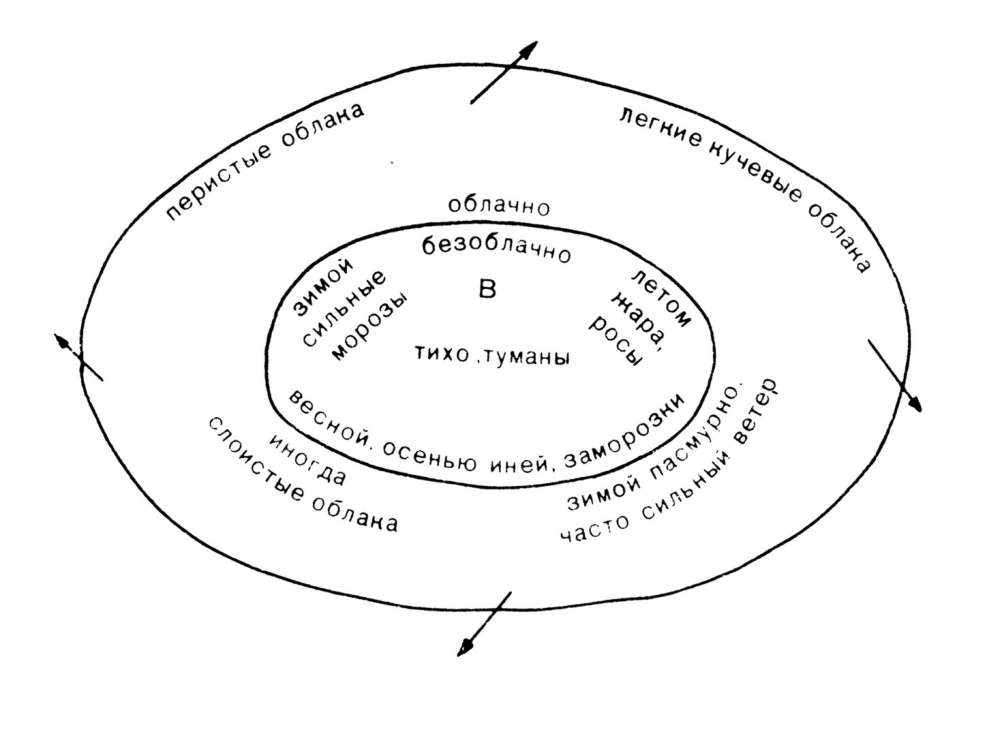
\includegraphics[scale=1.0]{04_anticyclon.pdf}
   \caption{Антициклон}
   \label{fig:04_anticyclon}
\end{figure*}

\textbf{Антициклон}\index{антициклон} \--- вихреобразное возмущение в
атмосфере с повышенным давлением в центре; область повышенного
атмосферного давления, состоящая из однородной воздушной массы
вращающейся по часовой стрелке в севером полушарии
(рис.~\ref{fig:04_anticyclon} и против часовой стрелки в южном
полушарии.

\section{Атмосферный фронт}
\label{sec:front}

\textbf{Атмосферный фронт}\index{атмосферный фронт} \--- сравнительно
узкая (несколько километров) переходная зона между двумя воздушными
массами.

Если воздушный поток направлен от тёплой воздушной массы к холодной,
то и фронт перемещается в этом направлении, такой фронт называется
\textbf{тёплым}\index{фронт!тёплый}.

\begin{figure*}[htb]
   \centering
   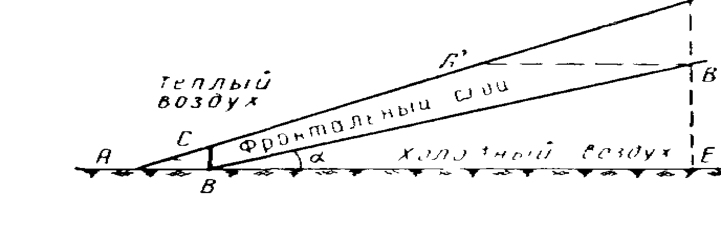
\includegraphics[scale=1.0]{05_vertical_front.pdf}
   \caption{Вертикальный разрез фронтального слоя}
   \label{fig:05_vertical_front}
\end{figure*}

Ширина фронтального слоя (рис.~\ref{fig:05_vertical_front} в приводном
(приземном) слое (отрезок $AB$) наименьшая: от нескольких до десятков
километров, а на высоте 3\otdo{}5~км ($A'B'$) может достигать
300~км. В верхней половине тропосферы ширина фронтальной зоны может
быть ещё больше. Вертикальная мощность слоя ($BC$ и $B'P$) обычно не
превышает 1~км. Горизонтальная проекция фронта $AE$ составляет
100\otdo{}1000~км, а его высота $EP$ \--- от 1 до 10~км.

Обычно толщиной фронтального слоя пренебрегают и считают, что фронт
\--- поверхность, которую называют фронтальной.

Различают следующие фронты: \textbf{основные}\index{фронт!основной}
(их называют тропосферными\index{фронт!тропосферный}, или
высокими\index{фронт!высокий}), \textbf{вторичные}\index{фронт!вторичный}
(приземные\index{фронт!приземный}, низкие\index{фронт!низкий}) и
\textbf{верхние}\index{фронт!верхний}.

Основными называются фронты, имеющие большую горизонтальную
(несколько тысяч километров) и вертикальную протяжённость. Эти фронты
разделяют воздушные массы, существенно отличающиеся по своим
свойствам.

Скачок температуры при переходе через линию основного фронта на
приземной карте обычно превышает 5\grC.

Вторичными называются фронты небольшой горизонтальной протяжённости,
(несколько сот километров).  Они разделяют различные порции одной и
той же воздушной массы. Высотная фронтальная зона со вторичными
фронтами не связана.

Верхними называются фронты, которые могут быть прослежены на картах
барической топографии, но не выявляются на приземных картах погоды.

Каждый основной фронт неоднороден по своим свойствам на всех
участках. Одни участки смещаются в сторону тёплой воздушной массы,
другие \--— в сторону холодной, третьи \--- малоподвижны. Поэтому фронты
классифицируются по ряду дополнительных признаков.

\section{Тёплый фронт}
\label{sec:warm_front}\index{фронт!тёплый}

\textbf{Тёплым} называются участки основного фронта, перемещающиеся в сторону
относительно холодной воздушной массы. За тёплым фронтом перемещается
тёплая воздушная масса.

\begin{figure*}[htb]
   \centering
   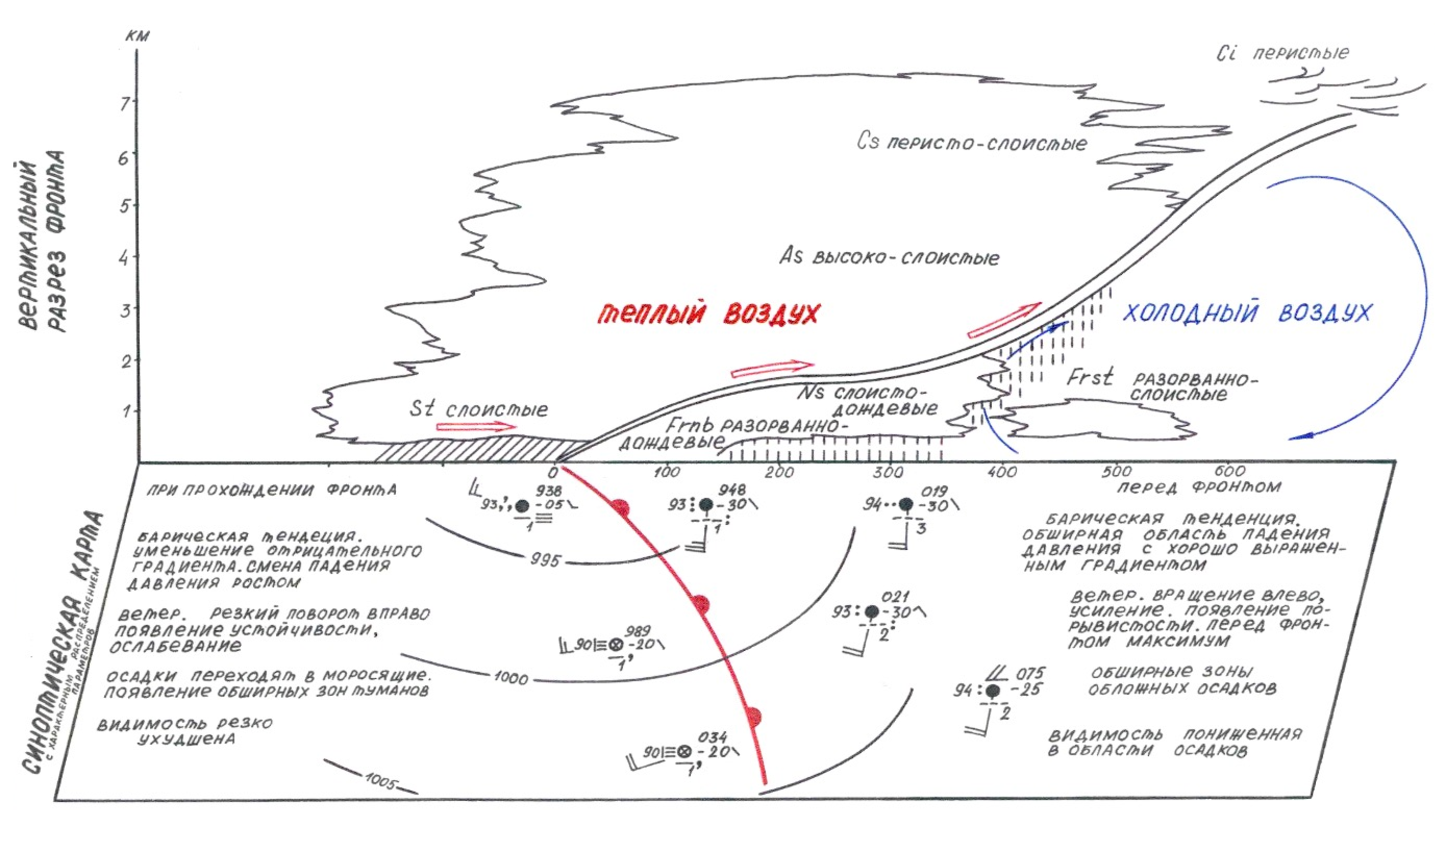
\includegraphics[scale=0.7]{06_warm_front.pdf}
   \caption{Тёплый фронт}
   \label{fig:06_warm_front}
\end{figure*}

Если фронт тёплый, то тёплый воздух натекает на холодный, поднимается
вверх над клином холодного воздуха и адиабатически
охлаждается. Содержащийся в нем водяной пар достигает насыщения и
конденсируется, образуя мощную облачную систему, состоящую из
слоисто-дождевых (\textit{Ns}), высоко-слоистых (\textit{Аs}) и
перисто-слоистых (\textit{Cs}) облаков, постепенно переходящих одни в
другие и образующих вместе как бы гигантский клинообразный массив,
сужающийся вперёд. Нижняя граница этого облачного массива
приблизительно совпадает с верхней границей фронтального слоя. Впереди
и несколько выше фронтальной поверхности обычно возникают перистые
облака (\textit{Ci}). Под поверхностью фронта в массах холодного
воздуха обычно образуются разорванно-слоистые (\textit{Frst}) облака.

На рис.~\ref{fig:06_warm_front} приведена схема вертикального строения
облачной системы тёплого фронта. Однако в каждом конкретном случае
строение облачной системы тёплых фронтов может существенно отличаться
от этой схемы.

Перед линией тёплого фронта образуется зона обложных
осадков\index{зона обложных осадков}, наибольшая ширина которой при
дожде достигает 300~км., а при снеге \--- 400~км. Это связано с тем,
что снег из высоко-слоистых облаков чаще достигает земной поверхности,
в то время как дождь в летнее время обычно при падении испаряется и до
земной поверхности не доходит. Внутри области осадков часто
наблюдается туман, обусловленный притоком водяного пара в холодный
воздух за счёт испарения осадков, а также адиабатическим охлаждением
воздуха в связи с падением давления. Ширина зоны тумана может
достигать 100\otdo{}200~км. Предфронтальный туман тёплого фронта чаще
всего образуется в холодное время года. Плохая видимость и сильный
ветер являются основными трудностями, которые могут встретиться при
пересечении тёплого фронта. Кроме того, зимой здесь возможно
обледенение судна.

После прохождения тёплого фронта наступает потепление. Вся система
облачности находится перед тёплым фронтом, поэтому по характеру
изменения облачности можно судить о приближении тёплого фронта.

При появлении перистых облаков начинается сначала медленное, а затем
постепенно ускоряющееся падение давления, которое прекращается
незадолго до прохождения линии фронта; после её прохождения давление
остаётся неизменным или медленно понижается, а иногда растёт.

Изменение скорости и направления ветра также является хорошим
признаком приближения тёплого фронта. По мере падения давления
скорость ветра постепенно увеличивается, достигая наибольшей величины
перед прохождением фронта. Направление ветра медленно отклоняется
влево, а в момент прохождения линии фронта резко поворачивает вправо
(в северном полушарии).

\section{Холодный фронт}
\label{sec:cold_front}\index{фронт!холодный}

\textbf{Холодными} называются участки основного фронта, перемещающиеся в
сторону относительно тёплой воздушной массы. За холодным фронтом
перемещается холодная воздушная масса.

Если воздушный поток направлен от холодной воздушной массы к более
тёплой, то такой фронт называется холодным. Отставание нижних слоев
воздуха от верхних под влиянием трения о земную поверхность приводит к
тому, что верхние слои обрушиваются вниз: холодный фронт приобретает
форму катящегося вала. Вытесняемый прямо вверх тёплый воздух быстро
поднимается и образует гряду тёмных туч \--- кучево-дождевых
облаков. В зависимости от скорости перемещения холодного воздуха
различают холодные фронты \textit{первого} (скорость передвижения
невелика, рис.~\ref{fig:07_cold_front_1}) и \textit{второго} рода
(рис.\ref{fig:08_cold_front_2}).

Структура холодных фронтов различается в зависимости от того, быстро
или медленно они движутся.

По этой причине различают: холодные фронты 1-го
рода\index{фронт!холодный 1-го рода} \--- медленно движущиеся фронты,
у которых облачность и осадки располагаются в основном за линией
холодные фронты 2-го рода\index{фронт!холодный 2-города} \--- быстро
движущиеся фронты, у которых облачность и осадки расположены в
основном перед линией фронта.

Холодные фронты 2-го рода наблюдаются в центральной части
циклона, а 1-го рода \--- на его периферии.

При холодном фронте 1-го рода происходит вытеснение масс тёплого
воздуха вторгающимся под него клином холодного воздуха. Здесь характер
облачности представляет собой зеркальное изображение облачности
тёплого фронта. Непосредственно перед линией фронта возникает
кучево-дождевые облака (\textit{Cb}), из которых выпадают ливневые осадки,
сопровождаемые грозами. Ширина зоны ливневой облачности \--- несколько
десятков километров.

\begin{figure*}[htb]
   \centering
   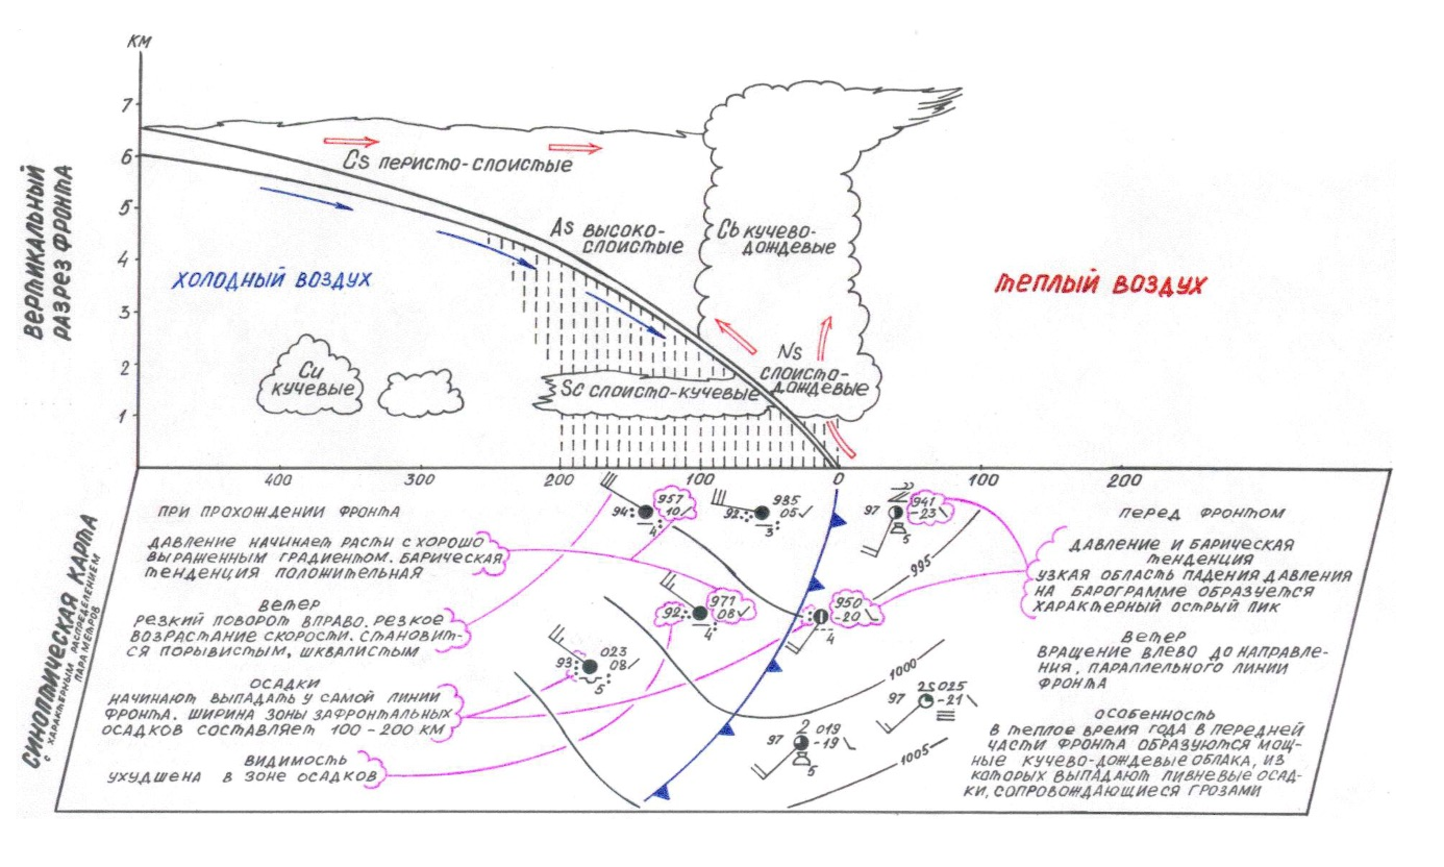
\includegraphics[scale=0.7]{07_cold_front_1.pdf}
   \caption{Холодный фронт 1-го рода}
   \label{fig:07_cold_front_1}
\end{figure*}

Облачная система \textit{Ns-As} с обложными осадками располагается за
линией фронта. Ширина зоны облачности, её мощность и, соответственно,
ширина зоны осадков примерно вдвое меньше, чем У тёплого фронта.

Таким образом, в отличие от тёплого фронта система облачности
холодного воздуха 1-го рода не позволяет заранее обнаружить его
приближение.

Холодный фронт 2-го рода отличается тем, что быстрое перемещение вала
холодного воздуха вызывает перед линией фронта бурный подъём
оттесняемого тёплого воздуха, а нисходящие движения воздушных потоков
препятствуют распространению облачной системы непосредственно за
линией фронта.

\begin{figure*}[htb]
   \centering
   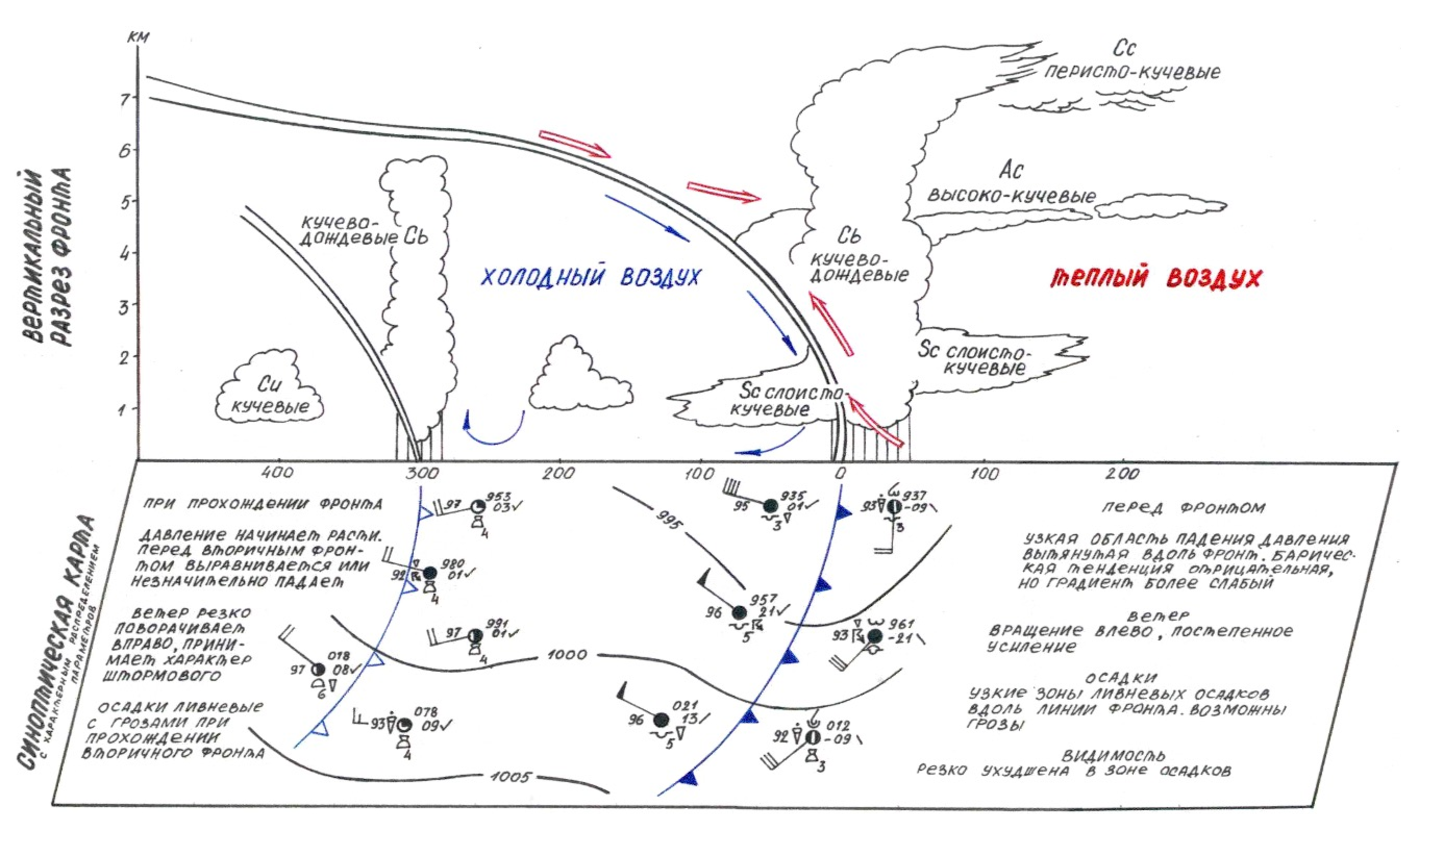
\includegraphics[scale=0.7]{08_cold_front_2.pdf}
   \caption{Холодный фронт 2-го рода}
   \label{fig:08_cold_front_2}
\end{figure*}

Возникающая облачная система представляет собой в основном вал мощных
облаков \textit{Cb}. При их растекании в небольшом количестве могут
образоваться \textit{Ci}, \textit{Cc}, \textit{Ac} и \textit{Sc}, а
под ними, в зоне выпадающих ливневых осадков, обычно наблюдаются
\textit{Cb} или \textit{Cu fra} (\textit{Cu fra} — разорванные
кучевые) плохой погоды.  На высотах 4\otdo{}5~км восходящий поток
адиабатически охлаждённого влажного воздуха встречается с нисходящим
потоком адиабатически нагретого сухого воздуха. В результате
образуется верхний вторичный фронт, под которым вал облаков
\textit{Cb} вытягивается вперёд. Передний его край, имеющий характер
\textit{Sc}, может постепенно разделиться на гряды чечевицеобразных
облаков \textit{Ac}. Эти облака выносятся вперёд от линии фронта на
200\otdo{}300 км и их обнаружение является надёжным предупреждением о
приближении холодного фронта 2-го рода.

Позади линии фронта в холодной массе воздуха наблюдаются нисходящие
движения воздуха, особенно значительные в передней части клина
холодного воздуха. Поэтому внутримассовые облака здесь не
возникают. Вскоре после прохождения линии фронта наступает быстрое
прояснение, вплоть до полного; лишь через несколько часов, когда
нисходящие движения затухнут и фронтальная поверхность достаточно
приподнимется, могут появиться свойственные холодной неустойчивой
массе конвективные облака и ливневые осадки.

Ливневые осадки при прохождении холодного фронта 2-го рода
непродолжительны (от нескольких минут до 1~ч), поскольку ширина зоны
осадков небольшая, а скорость перемещения фронта значительная.

В вале кучево-дождевых облаков холодного фронта 2-го рода иногда
встречаются разрывы или менее развитая облачность нижнего и среднего
ярусов. На отдельных участках фронта развивается грозовая
деятельность, которая, затухнув на одних участках, может появиться на
соседних.

Направление ветра при прохождении холодных фронтов обоих родов
изменяется так же, как и в случае тёплого фронта, но поворот вправо
(в северном полушарии) в момент прохождения линии холодного фронта \---
более значительный и резкий. Одновременно резко усиливается скорость
ветра.

При приближении холодного фронта наблюдается непродолжительное,
обычно слабое, но постепенно ускоряющееся падение давления. Тотчас по
прохождении линии фронта начинается рост давления, обусловленный
заменой тёплого воздуха холодным.

Температура воздуха после прохождения линии фронта понижается. Скачок
температуры зависит от характера сменяющихся масс.

Холодным фронтам обоих родов свойственны предфронтальные шквалы. Для
воздуха за холодным фронтом характерно нисходящее движение, которое
становится особенно интенсивным в передней части холодного клина, где
благодаря трению создаётся крутой наклон фронтальной
поверхности. Холодный воздух, обрушиваясь вниз, как бы перекатывается
вперёд, подобно гусеницам танка, причём скорость его продвижения
нормально к линии фронта во всех случаях оказывается больше, чем
соответствующая составляющая скорости тёплого воздуха в нижних
слоях. Обрушивание холодного воздуха приводит к вытеснению вверх
тёплого воздуха и к возникновению вдоль фронта вихря с горизонтальной
осью; с этим вихрем и связаны явления фронтальных шквалов.

Особенно интенсивное нисходящее движение имеет место в голове
холодного воздуха. Опускающийся с высоты нескольких километров, этот
воздух адиабатически нагревается, и благодаря этому скачок температуры
вдоль фронта сглаживается. В некоторых случаях внутри холодного клина
возникает вторичный холодный фронт, отделяющий нагревшийся воздух
<<головы>> от воздуха, лежащего дальше от линии фронта и не
захваченного в такой степени нисходящим движением.

Этот второй холодный фронт идёт на расстоянии нескольких километров за
размывшимся основным фронтом. При его прохождении наблюдается скачок
температуры, ветры и шквалы, но облачной системы он не имеет. Это
явление называют раздвоением холодного фронта.  В барических ложбинах
в тылу циклона обычно формируются вторичные холодные фронты. Причины
их образования будут рассмотрены ниже. Они имеют систему облаков,
сходную с системой облаков холодного фронта 2-го рода, однако
вертикальная протяжённость облаков меньше протяжённости облаков
основных холодных фронтов. В отдельных случаях может быть несколько
ложбин и вторичных фронтов.  Малоподвижными (стационарными) называются
участки основного фронта, не претерпевающие существенного
перемещения.

В циклоне холодный фронт перемещается несколько быстрее тёплого. С
течением времени происходит их сближение, а затем и слияние,
начинающееся близ центра циклона. Такой фронт, образовавшийся в
результате слияния холодного и тёплого фронтов, называется
\textbf{фронтом окклюзии}\index{фронт!окклюзии} (сомкнутым
фронтом\index{фронт!сомкнутый}).

Если холодный фронт догоняет идущий впереди него тёплый фронт;
холодный воздух, расположенный за холодным фронтом, смыкается с
холодным воздухом, расположенным перед тёплым фронтом, то такой
процесс называется окклюзией (окклюдированием) циклона, а сложный
фронт называется фронтом окклюзии. Скорость ветра в циклоне достигает
максимума непосредственно после начала окклюзии, циклон находится в
стадии максимального развития. В последующем наступает стадия
заполнения циклона. Атмосферное давление начинает расти, скорость
ветра уменьшаться.

\section{Фронты окклюзии}
\label{sec:ocl_front}

\textbf{Фронты окклюзии}\index{фронт!окклюзии} соединяют в себе черты
тёплого и холодного фронтов, но часто выражены менее резко.  В системе
фронтов окклюзии взаимодействуют три воздушные массы, из которых
наиболее тёплая уже не соприкасается с земной поверхностью. Поэтому,
помимо приземной линии, имеется линия верхнего фронта. При
образовании этого фронта может быть три случая:
\textit{нейтральная}\index{фронт!окклюзии!нейтральной},
\textit{тёплая}\index{фронт!окклюзии!тёплой} и
\textit{холодная}\index{фронт!окклюзии!холодной} окклюзия.

\textbf{Нейтральная}\index{фронт!окклюзии!нейтральной} имеет место,
когда массы холодного воздуха, движущиеся за холодным фронтом, имеют
одинаковую температуру с холодным воздухом, перемещающимся впереди
тёплого фронта. В момент смыкания холодных масс фронт отрывается от
земной поверхности и возникает верхний фронт. Характер облачности при
этом будет определяться системами облачности как тёплого, так и
холодного фронтов. В последующем будет происходить размывание
облачности и дальнейшее вытеснение тёплого воздуха вверх. Случай
нейтральной окклюзии очень редок, так как обычно температуры
отступающего и наступающего холодного воздуха неодинаковы. Иногда по
распределению температуры трудно судить о типе фронта окклюзии, в
связи с чем и было введено понятие окклюзии без уточнения. Часто
используются также термины: <<окклюзия по типу тёплого фронта>> и
<<окклюзия по типу холодного фронта>>.

Если холодный воздух за холодным фронтом оказывается теплее холодного
воздуха перед тёплым фронтом, то при прохождении линии фронта у
поверхности Земли будет отмечаться некоторое повышение температуры, и
в этом случае окклюзия называется \textbf{тёплой}
(рис.~\ref{fig:10_warm_ocl_front}). Характер облачности в начальный
момент одинаков с характером облачности при нейтральной окклюзии. В
последующем, в связи с тем, что холодный фронт перемещается быстрее
тёплого фронта, менее холодный воздух будет натекать на более
холодный. Массы тёплого воздуха вытесняются вверх, и образуются две
зоны раздела: верхний холодный и нижний тёплый фронты. По своим
внешним признакам тёплый фронт окклюзии сходен с тёплым фронтом. Все
признаки, относящиеся к тёплому фронту, справедливы и для тёплого
фронта окклюзии, однако они выражены значительно слабее.

\begin{figure*}[htb]
   \centering
   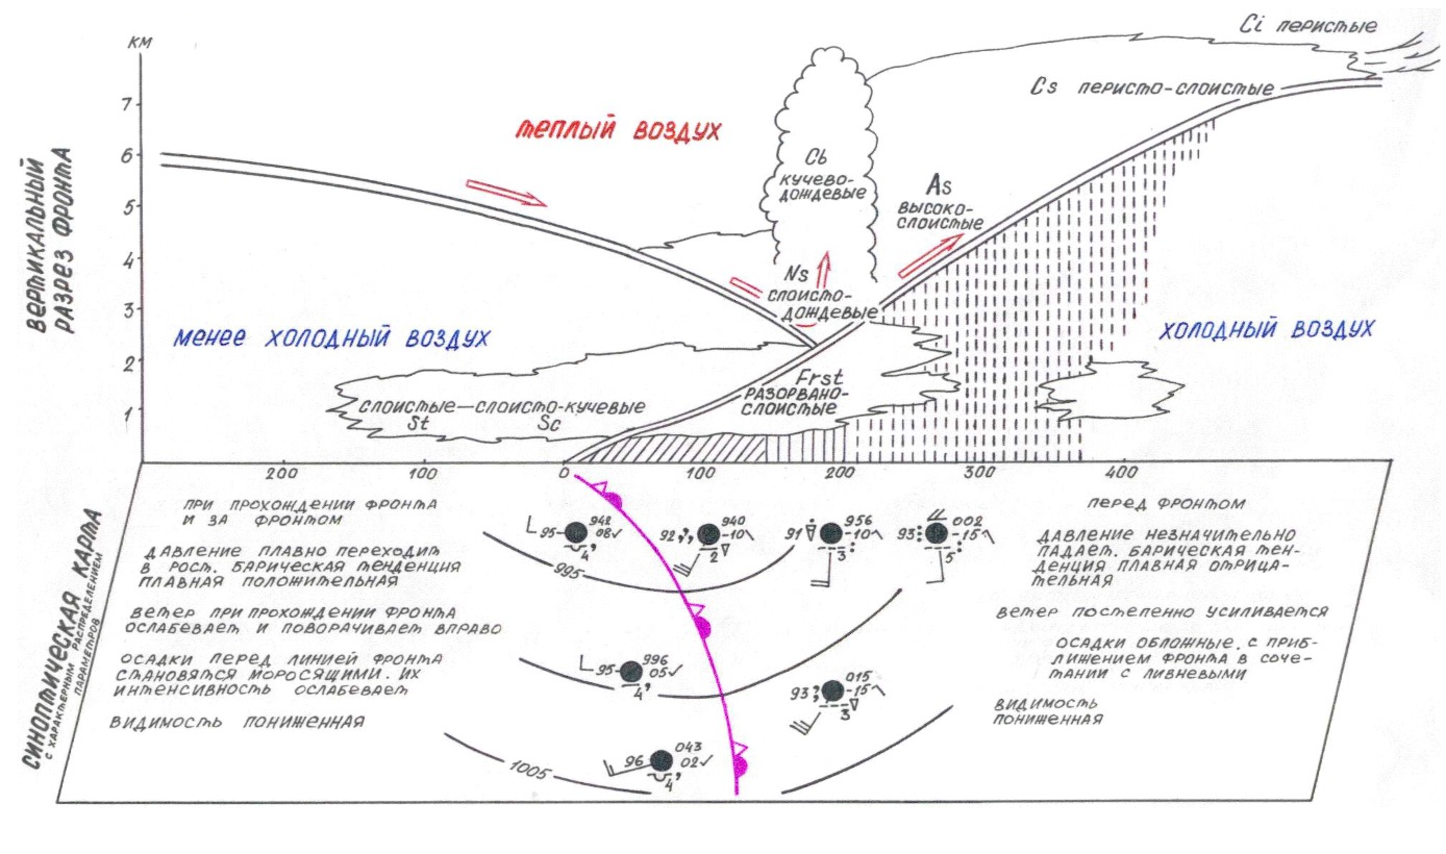
\includegraphics[scale=0.7]{10_warm_ocl_front.pdf}
   \caption{Фронт тёплой окклюзии}
   \label{fig:10_warm_ocl_front}
\end{figure*}

Если температура холодного воздуха за наступающим холодным фронтом
ниже температуры отступающего холодного воздуха перед тёплым фронтом,
то при прохождении линии фронта у поверхности Земли происходит
похолодание, и в этом случае окклюзия называется \textbf{холодной}
(рис.~\ref{fig:09_cold_ocl_front}). По всем внешним признакам холодный
фронт окклюзии сходен с холодным фронтом 1-го рода. Как и в предыдущем
случае, здесь также возникают две зоны раздела: верхний тёплый и
нижний холодный фронты.

\begin{figure*}[htb]
   \centering
   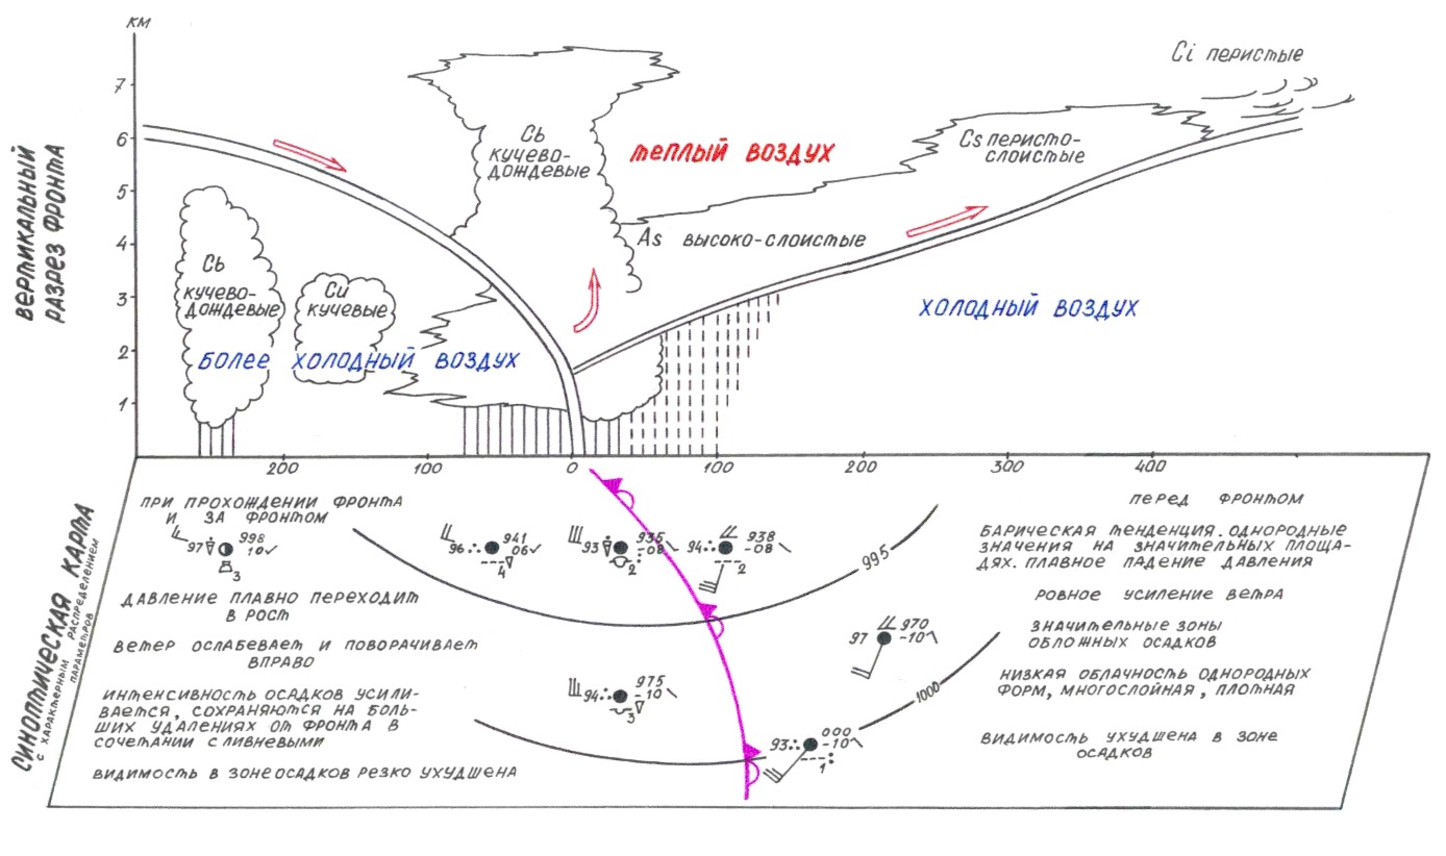
\includegraphics[scale=0.7]{09_cold_ocl_front.pdf}
   \caption{Фронт холодной окклюзии}
   \label{fig:09_cold_ocl_front}
\end{figure*}

Поскольку, как правило, верхний фронт расположен близко от приземного,
то на картах погоды практически их разграничить невозможно.

При прохождении фронта окклюзии направление ветра в северном полушарии
меняется по часовой стрелке, как и при прохождении тёплого или
холодного фронта.

Как при тёплой, так и при холодной окклюзии при небольшом контрасте
температур в массах холодного воздуха и при условии, что этот контраст
не усиливается, происходит размывание фронтов окклюзии. Если же
контраст температур достаточно большой или он усиливается, то
развивается облачность по типу тёплого или холодного фронтов.

В зависимости от соотношения температур воздуха по обе стороны фронта
окклюзии и направления его перемещения различают тёплые и холодные
фронты окклюзии. При одинаковой температуре по обе стороны фронт
окклюзии называется нейтральным.

По географической классификации различают следующие главные атмосферные фронты:
\textbf{арктический}\index{фронт!арктический}, разделяющий массы арктического и полярного (умеренного) воздуха;
\textbf{полярный}\index{фронт!полярный} (умеренный), разделяющий массы полярного (умеренного) и тропического воздуха;
\textbf{тропический}\index{фронт!тропический}, разделяющий массы тропического и экваториального воздуха.

\begin{figure*}[htb]
   \centering
   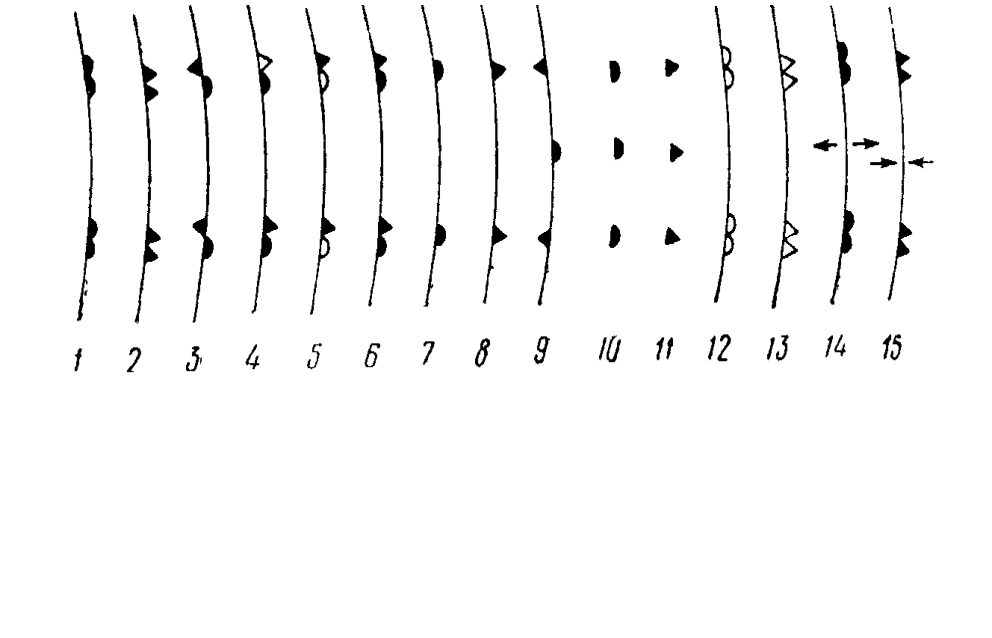
\includegraphics[scale=1]{11_fronts_marks.pdf}
   \caption{Фронт холодной окклюзии}
   \label{fig:fronts_marks}
   \small
   \begin{enumerate*}[itemjoin={{; }}, label={\arabic*~\--}]
   \item тёплый
   \item холодный
   \item малоподвижный
   \item тёплой окклюзии
   \item холодной окклюзии % 5
   \item нейтральной окклюзии
   \item тёплый размытый
   \item холодный размытый
   \item малоподвижный размытый
   \item тёплый вторичный % 10
   \item холодный вторичный
   \item тёплый верхний
   \item холодный верхний
   \item тёплый размывающийся
   \item холодный обостряющийся %15
   \end{enumerate*}
\end{figure*}

На рис.~\ref{fig:fronts_marks} показаны условные обозначения фронтов,
применяемые на фототелеграфных картах погоды.

Следует подчеркнуть, что рассмотренная схема отражает только главные
черты развития циклона. В действительности могут быть значительные
отклонения от этой схемы.

\section{Образование и размывание фронтов}
\label{sec:makes_fronts}

Фронты любого типа могут быть в одних случаях резко выраженными, или
\textbf{обостренными}\index{фронт!обострение}, в других случаях \--- слабо
выраженными, или \textbf{размытыми}\index{фронт!размытие}.

Если фронт \textit{обостренный}, то при переходе через его линию резко
изменяются температура воздуха и другие метеорологические элементы,
если \textit{размыт} \--— температура и другие метеорологические
элементы меняются постепенно.

Процессы образования и обострения фронтов называются
\textbf{фронтогенезом}\index{фронтогенез}, а процессы размывания
фронтов \--- \textbf{фронтолизом}\index{фронтолиз}. Эти процессы
наблюдаются непрерывно, подобно тому, как непрерывно формируются и
трансформируются воздушные массы.

Для образования фронта необходимо существование хотя бы небольшого
горизонтального градиента температуры и такого поля ветра, под
действием которого этот градиент значительно увеличился бы в некоторой
узкой полосе.

Особую роль в образовании и размывании фронтов играют \textit{барические
седловины} и связанные с ними \textit{деформационные поля ветра}. Если изотермы
в переходной зоне между соседними воздушными массами располагаются
параллельно оси растяжения или под углом менее 45\gr{} к ней, то в
деформационном поле происходит их сближение и горизонтальный
температурный градиент увеличивается. Наоборот, при расположении
изотерм параллельно оси сжатия или под углом менее 45\gr{} к ней
расстояние между ними увеличивается, и если уже сформированный фронт
попадет под такое поле, произойдет размывание фронта.

\section{Профиль фронтальной поверхности}
\label{sec:frontal_surface_profile}

Угол наклона \textbf{фронтальной поверхности} зависит от разности
температуры и скорости ветра теплой и холодной воздушной массы. На
экваторе фронты не пересекаются с земной поверхностью, а превращаются
в горизонтальные слои инверсии. Следует отметить, что на величину
наклона поверхности теплого и холодного фронтов некоторое влияние
оказывает трение воздуха о земную поверхность. В пределах слоя трения
скорость движения фронтальной поверхности с высотой увеличивается, а
выше уровня трения почти не изменяется. Это по-разному влияет на
профиль поверхности теплого и холодного фронтов. На рисунке
~\ref{fig:firction_sufrace_profile}\textit{a} линия \textit{I}
показывает первоначальное положение стационарного фронта с одинаковым
наклоном на всех уровнях.

\begin{figure*}[htb]
   \centering
   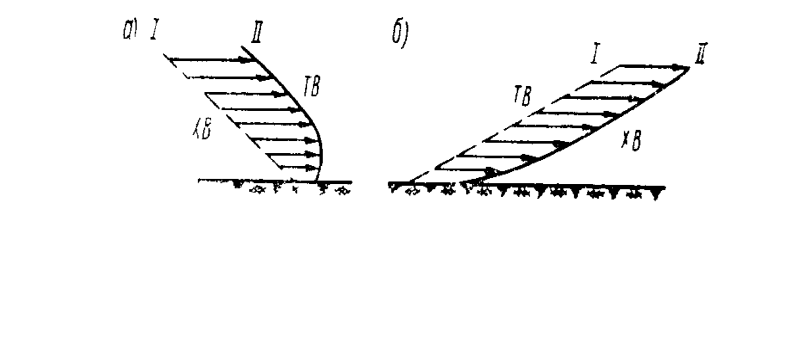
\includegraphics[scale=1]{12_friction_surface_profile.pdf}
   \caption[Влияние трения на профиль поверхностей]{Влияние трения на профиль поверхностей:}
   \label{fig:firction_sufrace_profile}
   \small
   \begin{enumerate*}[itemjoin={{; }}, label={}, after={{; }}]
   \item а \--- холодного фронта
   \item б \--- тёплого фронта
   \end{enumerate*}
   \begin{enumerate*}[itemjoin={{; }}, label={\Roman* \--- }]
   \item стационарный
   \item движущийся фронт
   \end{enumerate*}
\end{figure*}

Когда фронт начал смещаться как теплый, в том слое, где скорость
движения с высотой возрастает, фронтальная поверхность становится
более отлогой. Аналогичное построение для холодного фронта показывает,
что под влиянием трения нижняя часть поверхности холодного фронта
становится более крутой, чем верхняя, и даже может получить внизу
обратный наклон, так что теплый воздух у земной поверхности может
располагаться в виде клина под холодным.

\section{Перемещение фронтов}
\label{sec:fronts_moving}

Линии фронтов па картах погоды проходят вдоль осей барических
ложбин. Как известно, в ложбине линии тока имеют сходимость к оси
ложбины, а следовательно, к линии фронта. Поэтому при прохождении
фронта ветер довольно резко изменяет свое направление.

\textit{Вектор ветра} в каждой точке перед и за линией фронта можно
разложить на две составляющие: \textit{касательную} и
\textit{нормальную} к линии фронта. Для перемещения фронта имеет
значение лишь нормальная составляющая скорости ветра, величина которой
зависит от угла между изобарами и линией фронта. Скорость перемещения
фронтов может колебаться в весьма широких пределах, так как она
зависит не только от скорости ветра, но и от характера барического и
термического полей тропосферы в зоне фронта, а также от влияния
приземного трения. В среднем для теплых фронтов скорость перемещения
составляет $0,7$, а для холодных \--- около $0,8$ составляющей
геострофического ветра\footnote{Геостроф\'{и}ческий в\'{е}тер (от
  др.-греч. <<земля>> + <<поворот>>) — вызванный вращением Земли
  теоретический ветер, который является результатом полного баланса
  между силой Кориол\'{и}са и горизонтальным компонентом силы
  барического градиента — такие условия называются геострофическим
  балансом.}  у земной поверхности, нормальной к линии фронта.

Следует отметить, что сходимость ветров к линии фронта в приземном
слое стимулирует восходящие движения воздуха. Поэтому вблизи линий
фронтов имеются наиболее благоприятные условия для образования облаков
и выпадения осадков.

\section{Фронт и струйное течение}
\label{sec:front_and_stream}

В случае резкого фронта над ним и параллельно ему в верхней тропосфере
и нижней стратосфере наблюдается струйное течение, под которым
понимают узкие потоки воздуха с большими скоростями и большой
горизонтальной протяженностью. Максимальная скорость отмечается вдоль
мало наклоненной горизонтальной оси струйного течения. Длина
последнего измеряется тысячами, ширина \--- сотнями, толщина \---
несколькими километрами. Максимальная скорость ветра по оси струйного
течения составляет 30\mps{} и более.

Возникновение струйных течений связано с образованием в высотных
фронтальных зонах больших горизонтальных градиентов температуры,
обусловливающих, как известно, термический ветер.

Стадия молодого циклона продолжается до тех пор, пока в центре циклона
у земной поверхности остается теплый воздух. Продолжительность этой
стадии в среднем 12\otdo{}24~ч.

Обратим еще раз внимание, что как в начальной стадии развития, стадии
молодого циклона (рис.~\ref{fig:03_cyclon}) теплый и холодный фронты представляют собой два
участка волнообразно изогнутой поверхности основного фронта, на
которой развивается циклон.

В молодом циклоне можно выделить три зоны, резко отличающиеся по условиям погоды.

Зона \textit{I} \--- передняя и центральная части холодного сектора
циклона перед теплым фронтом. Здесь характер погоды определяется
свойствами теплого фронта Чем ближе к центру циклона и линии теплого
фронта, тем мощнее система облаков и тем вероятнее выпадение обложных
осадков наблюдается падение давления.

Зона \textit{II} \--- тыловая часть холодного сектора циклона за холодным
фронтом. Здесь погода определяется свойствами холодного фронта и
холодной неустойчивой воздушной массы. При достаточной влажности и
значительной неустойчивости воздушной массы выпадают ливневые
осадки. Атмосферное давление за линией холодного фронта растет.

Зона \textit{III} \--- теплый сектор. Поскольку теплая воздушная масса
является преимущественно влажной и устойчивой, то условия погоды в
ней обычно соответствуют условиям погоды в устойчивой воздушной массе.


\backmatter{}

\printindex

\end{document}

%%% Local Variables:
%%% mode: latex
%%% TeX-master: t
%%% End:
